% !BIB program = biber 
\documentclass{article}

%----------------------------------------------------------------------------------------
%	PACKAGES AND OTHER DOCUMENT CONFIGURATIONS
%----------------------------------------------------------------------------------------

% Generate dummy text (lorem ipsum) in your document
\usepackage{lipsum} % Comment me

% English language hyphenation
\usepackage[english]{babel}

% Math packages
\usepackage{amsmath, amsfonts, amsthm}

% Indent first paragraph
\usepackage{indentfirst}

% Figures
\usepackage{float}
\usepackage{graphicx}
\graphicspath{{./images/}}

% Captions
\usepackage{caption}
\usepackage{subcaption}

% Context sensitive quotation facilities
\usepackage{csquotes}

% Enumerate
\usepackage{enumitem}

% Chemical formulas package
\usepackage{chemformula}

% Filesystem
\usepackage{forest}

% Minted package for syntax highlighting
\usepackage{minted}

% Table 
\usepackage[toc]{appendix}
\addto\captionsenglish{% Replace "english" with the language you use
  \renewcommand{\contentsname}{Table of Contents}
}

% Shorthands
\usepackage{xspace}
\makeatletter
\DeclareRobustCommand\onedot{\futurelet\@let@token\@onedot}
\def\@onedot{\ifx\@let@token.\else.\null\fi\xspace}

\def\eg{e.g\onedot} \def\Eg{E.g\onedot}
\def\ie{i.e\onedot} \def\Ie{I.e\onedot}
\def\cf{cf\onedot} \def\Cf{Cf\onedot}
\def\etc{etc\onedot} \def\vs{vs\onedot}
\def\wrt{w.r.t\onedot} \def\dof{d.o.f\onedot}
\def\etal{et al.\onedot}
\makeatother

% Hyperlinks styling
\usepackage{hyperref}
% Hyperlink setup
\hypersetup{
  colorlinks   = true, % Colours links instead of ugly boxes
  urlcolor     = blue, % Colour for external hyperlinks
  linkcolor    = blue, % Colour of internal links
  citecolor    = blue, % Colour of citations
  linktocpage  = true, % Link only on page numbers
}
% PDF metadata
\hypersetup{
  pdftitle     = {Guia do usuário: Viabilidade celular},
  pdfauthor    = {Kayllany L. S. Oliveira, Daniel C. Vieira, José G. C. Pereira, João V. S. Guerra},
  pdfproducer  = {Latex with hyperref},
  pdfcreator   = {pdflatex}
}

% Bibliography
\usepackage[
  backend=biber,
  style=ieee,
  natbib=true,
]{biblatex}
\addbibresource{\jobname.bib}

% Acronyms
\usepackage[
  printonlyused,
  nohyperlinks,
  withpage,
]{acronym}

%----------------------------------------------------------------------------------------
%	DOCUMENT MARGINS
%----------------------------------------------------------------------------------------

\usepackage{geometry} % Required for adjusting page dimensions and margins
\geometry{
  paper=a4paper,
  top=30mm, % Top margin
  bottom=20mm, % Bottom margin
  left=30mm, % Left margin
  right=20mm, % Right margin
  % showframe, % Uncomment to show how the type block is set on the page
}

%----------------------------------------------------------------------------------------
%	FONTS
%----------------------------------------------------------------------------------------

% Required for inputting international characters
\usepackage[T1]{fontenc}
% Use 8-bit encoding
\usepackage[latin1,utf8]{inputenc}

% Fonts
\usepackage{lmodern}

% Title Page
\long\def\reporttitle{%
  \begin{titlepage}
    % Logo
    \begin{center}
      \begin{minipage}{0.9\textwidth}%

        
\includegraphics[width=\textwidth]{lnbio-cnpem-logo.png}%
      \end{minipage}
    \end{center}
    \vskip 1em

    % Horizontal line
    \hline
    \vskip 2em

      % Title
      {\centering \LARGE Guia do usuário: Viabilidade celular \par}
    \vskip 2em

      % Author
      {\centering \large Kayllany L. S. Oliveira, Daniel C. Vieira, José G. C. Pereira, João V. S. Guerra \par}
    \vskip 2em

      % Date
      {\centering \large \today\par}
    \vskip 1em

    % Horizontal line
    \hline

    % Do not break page
    \let\endtitlepage\relax
  \end{titlepage}
  
  % Version
  \vfill
  {\centering v1.0.0\par}
}

\begin{document}

% Make title
\reporttitle
\break

% Table of Contents
\hline
\tableofcontents
\vskip 0.5em
\hline
\break 

\section{Introdução}

Este guia do usuário fornece instruções detalhadas sobre como executar a análise de viabilidade celular. O objetivo deste guia é auxiliar os usuários a configurar e executar o pipeline de análise, bem como a interpretar os resultados obtidos.

\section{Requisitos}

Para executar a análise de viabilidade celular, você precisará dos seguintes requisitos:

\begin{itemize}
  \item \textbf{Acesso ao GitHub do CNPEM}: Você deve ter acesso ao repositório do projeto (\url{https://github.com/cnpem/CellViability}) no GitHub do CNPEM (\url{https://github.com/cnpem/}) para baixar os arquivos necessários. Se não tiver acesso, entre em contato com a Equipe de Dados Biológicos (\url{edb@lnbio.cnpem.br}).
  \item \textbf{Acesso ao HPCC Marvin}: Você deve ter acesso ao HPCC Marvin para executar o pipeline de análise. Se você não tiver acesso, acesse \url{https://marvindocs.cnpem.br/primeiros-passos/index.html}.
\end{itemize}

\section{Acessando o HPCC Marvin}

Para acessar o HPCC Marvin, comece abrindo o terminal. Se estiver usando Windows, abra o PowerShell; se estiver usando Linux ou MacOS, abra o Terminal. Para acessar o HPCC Marvin, use o comando:

\begin{minted}[frame=single, bgcolor=lightgray, fontsize=\small]{bash}
ssh <seu.login.cnpem>@marvin.cnpem.br
\end{minted}

Após inserir o comando, será solicitado que você insira sua senha, digite sua senha institucional.

\section{Preparando o Repositório \texttt{ParasiteCoLocalization}}

Para clonar o repositório \href{https://github.com/cnpem/CellViability}{CellViability}, execute o seguinte comando no terminal:

\begin{minted}[frame=single, bgcolor=lightgray, fontsize=\small]{bash}
git clone https://github.com/cnpem/CellViability.git
\end{minted}

O comando acima cria uma pasta chamada \texttt{CellViability} no diretório atual. Esta pasta contém todos os arquivos necessários para a execução da análise de viabilidade celular, incluindo o script \texttt{run.sh}, que automatiza a execução da análise via SLURM.

Após clonar o repositório \texttt{CellViability}, acesse o diretório do projeto com o comando:

\begin{minted}[frame=single, bgcolor=lightgray, fontsize=\small]{bash}
cd CellViability
\end{minted}

\subsection{Instalando PyEnv no HPCC Marvin}

O PyEnv é uma ferramenta que permite instalar e gerenciar várias versões do Python em um ambiente virtual. Para instalar o PyEnv no HPCC Marvin, execute os seguintes comandos no terminal:

\begin{minted}[frame=single, bgcolor=lightgray, fontsize=\small]{bash}
curl https://pyenv.run | bash
echo 'export PATH="$HOME/.pyenv/bin:$PATH"' >> ~/.bashrc
echo 'eval "$(pyenv init -)"' >> ~/.bashrc
echo 'eval "$(pyenv virtualenv-init -)"' >> ~/.bashrc
source ~/.bashrc
\end{minted}

Para instalar uma versão específica do Python, execute o seguinte comando:

\begin{minted}[frame=single, bgcolor=lightgray, fontsize=\small]{bash}
pyenv install 3.8.19
\end{minted}

Para definir a versão do Python como padrão neste diretório, execute o seguinte comando:

\begin{minted}[frame=single, bgcolor=lightgray, fontsize=\small]{bash}
pyenv local 3.8.19
\end{minted}

Caso deseje utilizar outra versão do Python, você pode selecionar a versão desejada para a sessão atual com o comando:

\begin{minted}[frame=single, bgcolor=lightgray, fontsize=\small]{bash}
pyenv shell <versão_desejada>
\end{minted}

\subsection{Instalando as Dependências do Python}

Para instalar as dependências do Python, execute o seguinte comando no terminal:

\begin{minted}[frame=single, bgcolor=lightgray, fontsize=\small]{bash}
pip install -r requirements.txt
\end{minted}

\subsection{Enviando Imagens para o HPCC Marvin}

Para enviar as imagens para o HPCC Marvin, você pode usar o comando \texttt{scp} em qualquer terminal.

\begin{minted}[frame=single, bgcolor=lightgray, fontsize=\small, breaklines]{bash}
scp /caminho/para/suas/imagens/*.tiff <seu.login.cnpem>@marvin.cnpem.br:/caminho/para/CellViability/data
\end{minted}

Caso você esteja usando o Windows, você pode usar o \href{WinSCP}{https://winscp.net/eng/download.php} para transferir arquivos de e para o HPCC Marvin. Para isso, siga as instruções abaixo:

\begin{enumerate}
  \item Abra o WinSCP e insira o endereço do servidor (\texttt{marvin.cnpem.br}), seu nome de usuário e senha.
  \item Navegue até o diretório \texttt{CellViability/data} no HPCC Marvin.
  \item Arraste e solte os arquivos de imagem do seu computador para o diretório \texttt{CellViability/data} no HPCC Marvin.
\end{enumerate}

\subsection{Executando o Pipeline no HPCC Marvin}

Após enviar as imagens para o HPCC Marvin, você pode executar o pipeline de análise de viabilidade celular. O script \texttt{run.sh} executa o pipeline de análise via SLURM, que é o sistema de gerenciamento de tarefas usado no HPCC Marvin. Para isso, execute o script \texttt{run.sh} no diretório \texttt{CellViability}.

\begin{minted}[frame=single, bgcolor=lightgray, fontsize=\small]{bash}
sbatch run.sh -m marvin
\end{minted}

O comando acima retorna o ID do job SLURM, que você pode usar para monitorar o progresso da análise.

\subsubsection{Monitoramento do Job SLURM}

Para monitorar o progresso do job SLURM, você pode usar o comando \texttt{squeue} no terminal. O comando \texttt{squeue} exibe informações sobre os jobs SLURM em execução no HPCC Marvin.

\begin{minted}[frame=single, bgcolor=lightgray, fontsize=\small]{bash}
squeue -u <seu.login.cnpem>
\end{minted}

Se o job estiver em execução, o estado será exibido como R (em execução). Se o job estiver aguardando na fila, o estado será PD (pendente).

Caso deseje cancelar o job SLURM, você pode usar o comando \texttt{scancel} no terminal. O comando \texttt{scancel} cancela um job SLURM em execução no HPCC Marvin.

\begin{minted}[frame=single, bgcolor=lightgray, fontsize=\small]{bash}
scancel <job_id>
\end{minted}

Por fim, você pode verificar o arquivo de log gerado pelo SLURM (\texttt{slurm\_<job\_id>.out}) para obter informações sobre o seu job.

\section{Visualizando os Resultados}

Após a conclusão da análise, os resultados serão armazenados no diretório \texttt{results/}, que incluem os seguintes arquivos:

\begin{itemize}
  \item \texttt{summary.csv}: Este arquivo contém um resumo dos resultados da análise por poço, incluindo contagem total de células.

\begin{minted}[frame=single, bgcolor=lightgray, fontsize=\footnotesize]{markdown}
|     | TotalCells |
| --- | ---------- |
| A1  | 487.0      |
| A2  | 217.0      |
| A3  | 863.0      |
| A4  | 58.0       |
| A5  | 180.0      |
| A6  | 54.0       |
| A7  | 296.0      |
| A8  | 227.0      |
\end{minted}
  
  \item \texttt{plate\_map/}: Este diretório contêm os mapas interativos da placa de 384 poços (Figura \ref{fig:plate_map}), contendo:

  \begin{itemize}
    \item \texttt{number\_of\_cells.html}: contagem total de células por poço.
  \end{itemize}

  \begin{figure}[H]
    \centering
    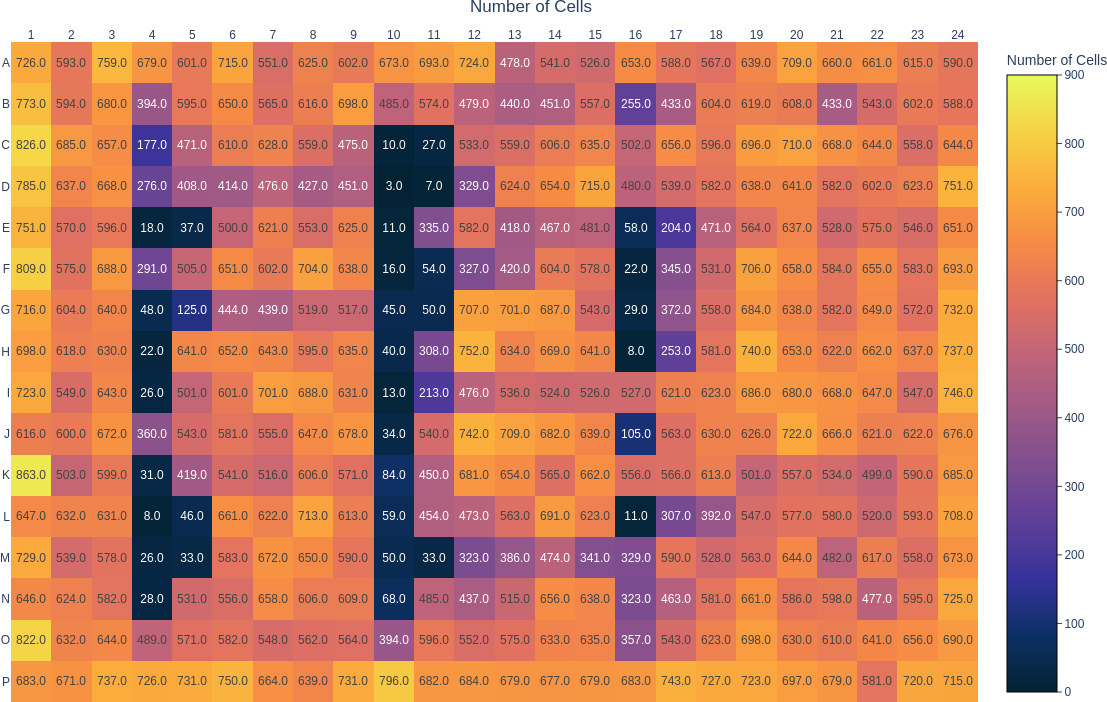
\includegraphics[width=0.65\textwidth]{images/example_plate_map.png}
    \caption{Exemplo de mapa interativo da placa de 384 poços.}
    \label{fig:plate_map}
  \end{figure}

\end{itemize}

\section{Ajustando o pipeline \texttt{parasitecolocalization.cppipe}}

\subsection{Entendendo e alterando o arquivo \texttt{cppipe} para ajustes na análise}
Dependendo dos dados que você está realizando, pode ser necessário ajustar o arquivo \texttt{cppipe} para configurar corretamente os módulos e as etapas do pipeline. Alterações no arquivo \texttt{cppipe} são importantes quando é necessário adaptar o pipeline para diferentes tipos de imagens ou análises.

Por exemplo, ao analisar células em imagens de alta resolução, pode ser necessário ajustar os parâmetros do módulo de segmentação para lidar com a maior resolução. Se estiver trabalhando com imagens de fluorescência, os parâmetros podem ser modificados para considerar o contraste ou a intensidade das células.

Para isso é preciso alterar o arquivo \texttt{cppipe}, que é um arquivo de configuração do CellProfiler que define a sequência de módulos a serem executados durante a análise de imagens, bem como os parâmetros específicos de cada módulo. Ele contém uma série de módulos que são executados sequencialmente, cada um realizando uma tarefa específica, como segmentação, medição ou visualização das imagens. Cada módulo possui parâmetros ajustáveis que controlam o comportamento da análise.



\subsection{Acessando o VNC para usar o CellProfiler}  

Para acessar o VNC e configurar o ambiente para executar o CellProfiler, siga os passos abaixo:  

\begin{enumerate}  
  \item Acesse o endereço \href{https://marvin.cnpem.br}{https://marvin.cnpem.br}.  
  \item Na aba \textbf{App Interativos}, selecione a opção \textbf{VNC}.  
  \item Na nova janela, configure os parâmetros:  
  \begin{itemize}  
    \item Escolha o número de horas que pretende utilizar.  
    \item Configure o número de GPUs necessárias \textbf{(Exemplo: 1, 2 e 3)}.  
    \item Selecione a opção \textbf{gui-gpu-small} como o perfil de GPU.  
  \end{itemize}  
  \item Clique em \textbf{Iniciar Sessão} para abrir o ambiente de VNC.  
\end{enumerate}  

Após o ambiente ser inicializado, abra o terminal e execute o seguinte comando para rodar o CellProfiler:  

\begin{minted}[frame=single, bgcolor=lightgray, fontsize=\small]{bash}  
singularity run --nv /opt/images/cellprofiler/cellprofiler-4_2_6.sif ~/Desktop/session.out  
\end{minted}  



\subsubsection{Editando o arquivo \texttt{cppipe} no CellProfiler}

O CellProfiler oferece tanto uma interface gráfica quanto uma de linha de comando para editar arquivos \texttt{cppipe}. Abaixo, detalhamos os passos para realizar edições utilizando a interface gráfica:

\begin{enumerate}
    \item \textbf{Abrir o CellProfiler}: Inicie o CellProfiler em sua máquina local ou no ambiente de trabalho.
    \item \textbf{Carregar o pipeline existente}: No menu inicial do CellProfiler, clique em 
    \texttt{Open Pipeline} e selecione o arquivo \texttt{cppipe} que deseja editar.
    \item \textbf{Modificar módulos e parâmetros}: O CellProfiler exibirá todos os módulos do pipeline na interface. Clique em qualquer módulo para visualizar e modificar seus parâmetros.
    \begin{itemize}
        \item Ajuste valores como \texttt{Thresholding} ou \texttt{Rescaling} no módulo de segmentação caso necessário.
        \item Para adicionar novos módulos, clique em \texttt{Add Module} e escolha o módulo apropriado.
    \end{itemize}
    \item \textbf{Salvar o novo pipeline}: Após realizar as alterações, clique em \texttt{Save Pipeline As} e salve o arquivo modificado.
    \item \textbf{Executar o pipeline}: Após salvar, execute o pipeline no CellProfiler ou via linha de comando, conforme descrito anteriormente.
\end{enumerate}

\subsubsection{Alterações comuns no arquivo \texttt{cppipe}}

Dependendo do tipo de análise e das características das imagens, você pode realizar alterações como:
\begin{itemize}
    \item Alterar o método de segmentação para lidar com diferentes características dos objetos nas imagens.
    \item Adicionar ou remover módulos para medir características específicas, como intensidade média das células.
    \item Ajustar os parâmetros de tamanho de objeto para considerar variações de tamanho das células.
    \item Modificar parâmetros de medição para analisar aspectos específicos, como área, intensidade ou forma.
\end{itemize}

\subsubsection{Testando o pipeline após alterações}

Após alterar o arquivo \texttt{cppipe}, é fundamental testá-lo com um conjunto representativo de imagens. Execute o pipeline em um subconjunto de imagens para garantir que os módulos estejam funcionando corretamente e que as medições estejam adequadas. Isso ajuda a identificar e corrigir rapidamente problemas antes de aplicar o pipeline ao conjunto completo de dados.

\printbibliography

\end{document}
